\documentclass[t,10pt,hyperref={
  %pdfpagemode=FullScreen,
  pdftitle = {gearshifft},
  pdfsubject = {gearshifft},
  %linktocpage=true,
  pdfborder={0 0 0},
  colorlinks=true,
  urlcolor=red,
  citecolor=red,
  linkcolor=red,
  pdfauthor={Peter Steinbach, Matthias Werner}
  }
]{beamer}
\usetheme{custom}
\def\resetbeamertemplate{\setbeamertemplate{background canvas}{ }}
\let\Tiny=\tiny
%\usepackage{lmodern}
\usepackage{tikz}
\usetikzlibrary{matrix}
\usetikzlibrary{calc}
\usetikzlibrary{positioning}
\usetikzlibrary{arrows}
\usetikzlibrary{trees}

\usepackage[utf8]{inputenc}
\usepackage[T1]{fontenc}
\usepackage{csquotes}
\usepackage{ifthen}

\usepackage{amsmath,amstext,amsthm,array,booktabs}
\usepackage{caption}
\usepackage{xcolor}
\usepackage{graphicx}
\usepackage{colortbl}
\usepackage{listings}
\usepackage{dirtree}

\usepackage[%per=slash,
%            decimalsymbol=comma,
            locale=US,
            ]{siunitx}

%%%%%%%%%%
\providecommand\thispdfpagelabel[1]{}


\lstset{literate={~} {$\sim\,$}{1}}
\lstset{upquote=true}
\lstset{language=C++,
  basicstyle=\small\fontfamily{fvm}\selectfont,%\ttfamily,
% 	columns=fullflexible,
  columns=fixed,
  keepspaces=true,
%       keywordstyle=\color{black}\bf,
%       stringstyle=\color{red}\ttfamily,
  showstringspaces=false,
  commentstyle=\color[rgb]{0.3,0.3,0.3}\textit,
%       morecomment=[l][\color{gray}]{\#},
  identifierstyle=\color{black},
  morekeywords={size_t},
  emph={__global__,__device__},
        emphstyle=\textit,
        numbers=left,
  numberstyle=\small\color{gray},
  breaklines=true,
  numbersep=5pt,
  xleftmargin=.19in,
}
% %%%%%%%%%%%%%%%%%%%%%%%%%%%%%%%%%%%%%%%%%%%%%%%%%%%%%%%%%%%%%%%%%%%%%%%%%%%%%%%

% \mode<presentation>{%
% \setbeameroption{show notes}
% }

\newcolumntype{M}{>{$\displaystyle}l<{$\vspace{1ex}}}
\title{gearshifft -- The FFT Benchmark Suite for Heterogeneous Platforms}
% \author{
%   \parbox{0.44\textwidth}{%\centering %
%     Peter Steinbach\\[.5em]
%     {\footnotesize{Max Planck Institute of Molecular Cell Biology and Genetics}}\\
%     {\small{01307 Dresden, Germany\\
%     \url{steinbac@mpi-cbg.de}}}}
% \hfill
% \parbox{0.47\textwidth}{
%   Matthias Werner\\[.5em]
% {\footnotesize{Center for Information Services and High Performance Computing}}\\
% {\small{TU Dresden, Germany\\
% \url{Matthias.Werner1@tu-dresden.de}}}}
% }
\author[Steinbach, Werner]{\texorpdfstring{%
    \begin{minipage}[b]{.5\textwidth}
      \centering
      Peter Steinbach\\[.5em]
      {\footnotesize{Max Planck Institute of Molecular Cell Biology and Genetics\\
          01307 Dresden, Germany}}\\
      {\small{\url{steinbac@mpi-cbg.de}}}
    \end{minipage}%
    \begin{minipage}[b]{.5\textwidth}
      \centering
      Matthias Werner\\[.5em]
      {\footnotesize{Center for Information Services and High Performance Computing\\
          TU Dresden, Germany}}\\
      {\small{\url{Matthias.Werner1@tu-dresden.de}}}
    \end{minipage}}{The Author}}

\date{2017/06/20}

%%%%%%%%%%%%%%%%%%%%%%%%
\tikzset{class/.style={inner sep=5pt,font=\footnotesize}}
\newcommand{\pclass}[5][]{
\ifthenelse { \equal {#1} {} }
 {\node[class] (#5) at (#3,#4) {#2};}
 {\node[class] (#5) at (#3,#4) {%
\begin{tabular}{c}\scriptsize{<<#1>>}\\{\textbf{#2}}\end{tabular}%
};}
}
\newcommand{\tkzgearshifft}{
%align=center,rounded corners,inner sep=5pt,rectangle,draw,
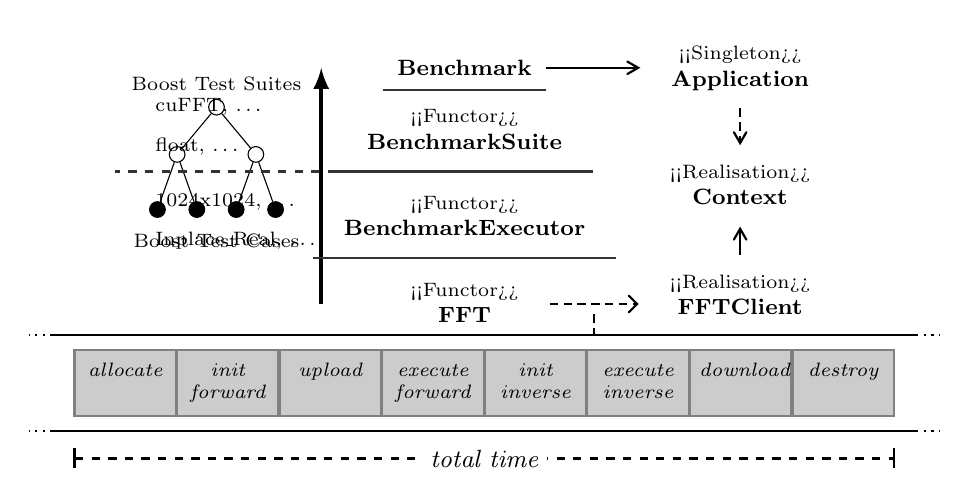
\begin{tikzpicture}
\tikzset{gr1/.style={}}
\tikzset{bts/.style={draw,circle,inner sep=2pt}}
\tikzset{btc/.style={draw,circle,inner sep=2pt,fill=black}}
%
\visible<1>{
\begin{scope}[yshift=3.5cm,xshift=-3.4cm]
\node[bts] (b0) at (0,0) {};
\node[bts] (b10) at (-0.5,-0.6) {}; \draw (b10) -- (b0);
\node[bts] (b11) at (0.5,-0.6) {}; \draw (b11) -- (b0);
\node[btc] (b20) at (-0.75,-1.3) {}; \draw (b20) -- (b10);
\node[btc] (b21) at (-0.25,-1.3) {}; \draw (b21) -- (b10);
\node[btc] (b22) at ( 0.25,-1.3) {}; \draw (b22) -- (b11);
\node[btc] (b23) at ( 0.75,-1.3) {}; \draw (b23) -- (b11);
\node[font=\scriptsize] at (0, 0.3) {Boost Test Suites};
\node[font=\scriptsize] at (0,-1.7) {Boost Test Cases};
\draw[ultra thick,-latex] (1.33,-2.5) -- ++(0,3.0);
\end{scope}}\visible<2>{
\begin{scope}[yshift=3.5cm,xshift=-4.3cm,every node/.style={anchor=west,align=left,font=\scriptsize}]
\node at (0,0) {cuFFT, \ldots};
\node at (0,-0.5) {float, \ldots};
\node at (0,-1.2) {1024x1024, \ldots};
\node at (0,-1.7) {Inplace\_Real, \ldots};
\end{scope}}

% 
\begin{scope}[xshift=1.75cm]
\begin{scope}
\pclass{{\textbf{Benchmark}}}{-2}{4}{b}
\pclass[Functor]{BenchmarkSuite}{-2}{3.2}{bs}
\pclass[Functor]{BenchmarkExecutor}{-2}{2.1}{be}
\pclass[Functor]{FFT}{-2}{1.0}{fft}
\end{scope}
\begin{scope}
\pclass[Singleton]{Application}{1.5}{4}{app}
\pclass[Realisation]{Context}{1.5}{2.5}{ctx}
\pclass[Realisation]{FFTClient}{1.5}{1.1}{impl}
\end{scope}
\end{scope}
\matrix[
 minimum height=1.5em,
 matrix of nodes,
 row sep=-\pgflinewidth,
 ampersand replacement=\&,
 column sep=-\pgflinewidth,
 text depth=2.5ex,
 text height=1.5ex,
 text width=3.0em,
 align=center,
 nodes in empty cells,
 row 1/.style={nodes={fill=black!20,draw=black!50,thick,rectangle,draw,minimum width=2.5em,font=\scriptsize\itshape}}
]
(mf) at (0,0) {
allocate \&
init\linebreak forward \&
|[gr1]| upload \&
|[gr1]| execute\linebreak forward \&
init\linebreak inverse \&
|[gr1]| execute\linebreak inverse \&
|[gr1]| download \&
destroy\\
};
\begin{scope}[thick]
\draw (mf-1-1.north west) ++(-0.75em,0.5em) coordinate (ctl) -- ([xshift=0.75em,yshift=0.5em]mf-1-8.north east) coordinate (cr);
\draw[dotted] (ctl) -- ++(-2ex,0); \draw[dotted] (cr) -- ++(2ex,0);
\draw (mf-1-1.south west) ++(-0.75em,-0.5em) coordinate (cl) -- ([xshift=0.75em,yshift=-0.5em]mf-1-8.south east) coordinate (cr);
\draw[dotted] (cl) -- ++(-2ex,0); \draw[dotted] (cr) -- ++(2ex,0);
% total time
\draw[thick,dashed,|-|] (mf-1-1.south west) ++(0,-1.5em) -- ([yshift=-1.5em]mf-1-8.south east) node[pos=0.5,fill=white,font=\small\itshape] {total time};
% (mf-1-1.south west) -- ++(0,-1.5em) -| (mf-1-8.south east) node[pos=0.25,fill=white,font=\small] {total time};

% \draw[-latex] (b) -- (bs);
% \draw[-latex] (fft) -- (ctl-|fft);
\draw[black!80] (b.south west) -- (b.south east);
\draw[black!80] (bs.south west) -- (bs.south east);
\draw[black!80, dashed] (bs.south west) -- ++(-8em,0); % test suite marker
\draw[black!80] (be.south west) -- (be.south east);

\draw[densely dashed,-angle 60] (app) -- (ctx);
\draw[-angle 60] (b) -- (app.west|-b);
\draw[-angle 60] (impl) -- (ctx.south);
% \draw[densely dashed,-angle 90] (be.east) -| (impl.north);
% \draw[densely dashed,-open triangle 60] (impl) -- (fft.east|-impl) node[midway] (q) {};
\draw[densely dashed,-angle 90] (fft) -- (impl.west|-fft) node[midway] (q) {};
\draw[densely dashed] (q) -- (ctl-|q);
\end{scope}
\end{tikzpicture}
}
%%%%%%%%%%%%%%%%%%%%%%%%%%%%
\definecolor{arccl}{rgb}{0.45,0.45,0.45}
\newcommand{\mgraymidrule}{\arrayrulecolor{arccl}\midrule\arrayrulecolor{black}}
%%%%%%%%%%%%%%%%%%%%%%%%%%%%%%%%%%%%%%%%%%%%%%%%%%%%%%%%%%%%%%%%%%%%%%%%




\newcommand{\gearshifft}{\texttt{gearshifft}}
\newcommand{\fftw}{\texttt{fftw}}
\newcommand{\cufft}{\texttt{cuFFT}}
\newcommand{\clfft}{\texttt{clFFT}}
\newcommand{\nvidia}{Nvidia}
\newcommand{\mc}[1]{\lstinline!#1!}
\newcommand{\iu}{{\mathrm{i}\mkern1mu}}

%%
\begin{document}
\frame[plain]{\titlepage}

\begin{frame}{Introduction}{FFTs}

  \begin{equation}
    \label{eq:dft}
    \text{DFT: }\quad X[k] = \sum_{j=0}^{n-1} x[j]\cdot\exp\left(\frac{-2\pi \iu jk}{n}\right),\quad x,X\in\mathbb{C}^n
  \end{equation}
  
  \begin{itemize}
  \item fast implementation of the discrete Fourier transform (DFT) \eqref{eq:dft}
  \item forward transform: time domain $\Rightarrow$ frequency domain
  \item by factorization of $n$ and recursive decomposition smaller DFTs are computed with $\mathcal{O}(n\log n)$
  \item Cooley-Tukey: Radix-2 DFTs
  \item Stockham's formulations avoids incoherent memory access
  \item Bluestein's algorithm allows arbitrary and mixed radices
%  \item FFT libraries fftw, clFFT, cuFFT, \ldots 
  \end{itemize}

\end{frame}

\begin{frame}{FFTs}
  \centering
  \begin{tikzpicture}
    \begin{scope}[every node/.style={align=center, anchor=north}, xscale=1.15, yscale=2.5]
      \node[fill=yellow,inner sep=5pt,draw,rectangle,rounded corners] at (0,-0.5) {\textbf{FFTs}};
      % https://commons.wikimedia.org/wiki/File:JPEG_compression_Example.jpg
      \node at (-3, 0.0) {\includegraphics[width=0.25\textwidth]{jpeg-compression.jpg}\\ compression};
      % https://imagej.net/Multiview-Reconstruction
      \node at ( 3, 0.0) {\includegraphics[width=0.25\textwidth]{imagej.jpg}\\ biology};
      % https://commons.wikimedia.org/wiki/File:Deep_learning.png
      \node at (-3, 1.0) {\includegraphics[width=0.21\textwidth]{deep-learning.png}\\ machine learning};
      % https://en.wikipedia.org/wiki/Trader_%28finance%29#/media/File:Philippine-stock-market-board.jpg
      \node at ( 3, 1.0) {\includegraphics[width=0.25\textwidth]{Philippine-stock-market-board.jpg}\\ financial math};
      % https://de.wikipedia.org/wiki/Sinc-Funktion#/media/File:Si_sinc.svg
      \node at ( 0, 1.0) {\includegraphics[width=0.25\textwidth]{sin-cos.png}\\ signal processing};
      % https://en.wikipedia.org/wiki/Interferometry#/media/File:USA.NM.VeryLargeArray.02.jpg
      \node at (-3,-1.0) {\includegraphics[width=0.25\textwidth]{usa-nm-vla.jpg}\\ astronomy};
      \node at ( 0,-1.5) {\Large\textbf{\ldots}};
      % https://en.wikipedia.org/wiki/Geology_applications_of_Fourier_transform_infrared_spectroscopy#/media/File:FTIR_spectrum.jpg
      \node at ( 3,-1.0) {\includegraphics[width=0.25\textwidth]{FTIR_spectrum.jpg}\\ geology};
    \end{scope}
  \end{tikzpicture}
\end{frame}

\begin{frame}{FFTs}
  \centering  
  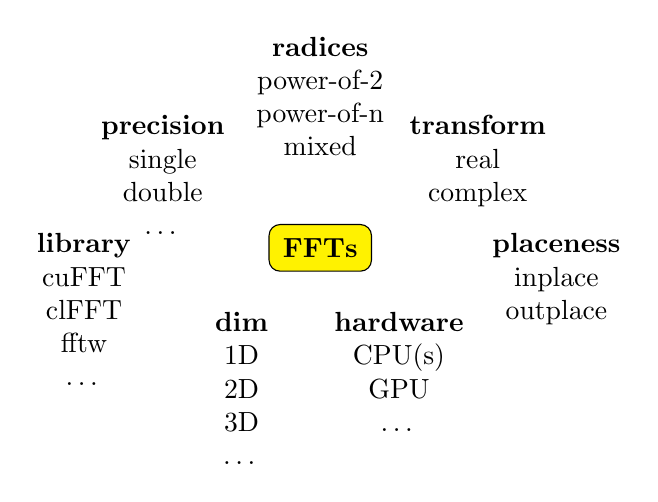
\begin{tikzpicture}
    \begin{scope}[every node/.style={align=center, anchor=north}]
      \node[fill=yellow,inner sep=5pt,draw,rectangle,rounded corners] {\textbf{FFTs}};
    \node at (-3, 0.0) {\textbf{library}\\ cuFFT\\ clFFT\\ fftw\\ \ldots};
    \node at ( 3, 0.0) {\textbf{placeness}\\ inplace\\ outplace};
    \node at (-2, 1.5) {\textbf{precision}\\ single\\ double\\ \ldots};
    \node at ( 2, 1.5) {\textbf{transform}\\ real\\ complex};
    \node at ( 0, 2.5) {\textbf{radices}\\ power-of-2\\ power-of-n\\ mixed};
    \node at (-1,-1.0) {\textbf{dim}\\ 1D\\ 2D\\ 3D\\ \ldots};
    \node at ( 1,-1.0) {\textbf{hardware}\\ CPU(s)\\ GPU\\ \ldots};
    \end{scope}
  \end{tikzpicture}

  \pause

  $\Rightarrow$ \textbf{Which FFT implementation works best on what hardware?}

\end{frame}


\begin{frame}{gearshifft}{Basic Framework in C++/Boost}
\tkzgearshifft
\end{frame}

\definecolor{mc1}{rgb}{0.0, 0.0, 1.0}
\definecolor{mc2}{rgb}{0.0, 0.5, 0.5}
\definecolor{mc3}{rgb}{0.5, 0.0, 0.0}
\begin{frame}[fragile]{gearshifft}
  cmake-based C++11/14 project:
\dirtree{%
.1 {gearshifft}.
.2 {config}\DTcomment{config files with FFT extents}.
.2 {inc}.
.3 \color{mc1}{core}\DTcomment{benchmark suite header files}.
.3 \color{mc3}{libraries}\DTcomment{FFT library instantiations}.
.4 \color{mc3}{cufft}.
.4 \color{mc3}{clfft}.
.4 \color{mc3}{fftw}.
.4 \color{mc3}{\ldots}.
.2 {src}.
}

\vfill

gearshifft run examples:
\begin{lstlisting}[numbers=none]
./gearshifft_clfft -f ../config/extents.csv
                   -o result.csv -d gpu -n 0
./gearshifft_clfft -e 1048576
                   -r */float/*/Outplace_Real
\end{lstlisting}

\end{frame}


\end{document}

%%% Local Variables:
%%% mode: latex
%%% TeX-master: t
%%% End:
